\documentclass[dvisvgm, tikz, border=4pt]{standalone}
\begin{document}
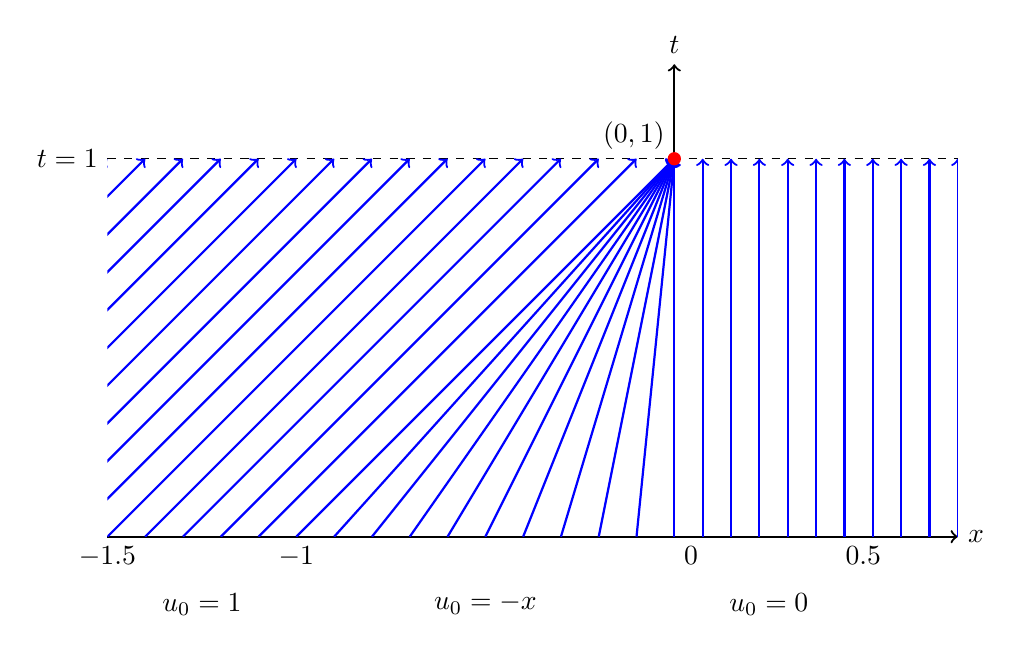
\begin{tikzpicture}[scale=1.2]
  % Display coordinates: X=4x, T=4t.
  \draw[->,thick] (-6,0) -- (3,0) node[right] {$x$};
  \draw[->,thick] (0,0) -- (0,5) node[above] {$t$};

  \draw[dashed] (-6,4) -- (3,4);
  \node[left] at (-6,4) {$t=1$};

  \begin{scope}
    \clip (-6,0) rectangle (3,4);

    % Left parallel characteristics.
    \foreach \k in {0,...,15}{
      \pgfmathsetmacro{\a}{-10+0.4*\k}
      \draw[blue,thick,->] (\a,0) -- ({\a+4},4);
    }

    % Compressing characteristics.
    \foreach \k in {1,...,9}{
      \pgfmathsetmacro{\a}{-4+0.4*\k}
      \draw[blue,thick,->] (\a,0) -- (0,4);
    }

    % Right parallel characteristics.
    \foreach \k in {0,...,15}{
      \pgfmathsetmacro{\a}{0.3*\k}
      \draw[blue,thick,->] (\a,0) -- (\a,4);
    }
  \end{scope}

  % Shock formation.
  \fill[red] (0,4) circle (2pt);
  \node[above left] at (0,4) {$(0,1)$};

  % Physical coordinates.
  \node[below] at (-6,0) {$-1.5$};
  \node[below] at (-4,0) {$-1$};
  \node[below right] at (0,0) {$0$};
  \node[below] at (2,0) {$0.5$};

  % Initial data.
  \node[below] at (-5,-0.5) {$u_0=1$};
  \node[below] at (-2,-0.5) {$u_0=-x$};
  \node[below] at (1,-0.5) {$u_0=0$};
\end{tikzpicture}
\end{document}
